\documentclass[11pt]{amsart}
\usepackage{geometry}                % See geometry.pdf to learn the layout options. There are lots.
\geometry{letterpaper}                   % ... or a4paper or a5paper or ... 
%\geometry{landscape}                % Activate for for rotated page geometry
%\usepackage[parfill]{parskip}    % Activate to begin paragraphs with an empty line rather than an indent
\usepackage{graphicx}
\usepackage{amsmath}
\usepackage{amssymb}
\usepackage{epstopdf}
\usepackage[framed,numbered,autolinebreaks,useliterate]{mcode}
\DeclareGraphicsRule{.tif}{png}{.png}{`convert #1 `dirname #1`/`basename #1 .tif`.png}

\title{Scientific Computing Homework 3}
\author{Howard Jing, Sun Hyoung Sonya Kim}
\date{November 7, 2011}                                           % Activate to display a given date or no date

\begin{document}
\maketitle
%\section{}
\subsection*{6.1}

The root x$_{\star}$ = 0 is degenerate because for $f(x)$ = x$^{2}$, $f'(x)$ = $2x$ and $f'$(x$_{\star}$)=2(0) = 0. To show $|$x$_{k+1}$-x$_{\star}$$|$ $\approx$ $\alpha$$|$x$_{k}$-x$_{\star}$$|$, we taylor expand $f$(x$_{k}$) and $f'$(x$_{k}$) around x$_{\star}$. 
\[
f(x_{k}) = f(x_{\star})+f'(x_{\star})(x_{k}-x_{\star})+\frac{f''(x_{\star})}{2}(x_{k}-x_{\star})+ ...
\]
\[
f'(x_{k}) = f'(x_{\star})+f''(x_{\star})(x_{k}-x_{\star})+...
\]
\newline
Subtract x$_{\star}$ from each side of the Newton iteration equation, and plug in the expansion 
\[
x_{k+1}-x_{\star}=x_{k}-x_{\star}-\frac{f(x_{k})}{f'(x_{k})}
\]
\[
x_{k+1}-x_{\star} = x_{k}-x_{\star}-\frac{f(x_{\star})+f'(x_{\star})(x_{k}-x_{\star})+\frac{f''(x_{\star})}{2}(x_{k}-x_{\star})+ ...}{f'(x_{\star})+f''(x_{\star})(x_{k}-x_{\star})+...}
\]
\newline
Since $f$(x$_{\star}$) = 0 and $f'$(x$_{\star}$) = 0, the above equation becomes
\[
x_{k+1}-x_{\star} \approx x_{k}-x_{\star}-\frac{x_{k}-x_{\star}}{2}
\]
\[
x_{k+1}-x_{\star} \approx \frac{1}{2}(x_{k}-x_{\star})
\]
\newline
Thus we have shown that there is an $\alpha$ $<$1 with $|$x$_{k+1}$-x$_{\star}$$|$ $\approx$ $\alpha$$|$x$_{k}$-x$_{\star}$$|$.
\newline
\newline
In contrast, quadratic local convergence for a non degenerate problem implies that there is a C$>$0 such that $|$$f$($x$$'$)$|$ $\le$ C $\cdot$ $|$$f$($\bar{x}$)$|$$^{2}$. Therefore the residual at the next iterations is proportional to the square of the residual at the current iterate whereas in the degenerate case, the residual at the next iteration is roughly proportional to the residual at the residual at the current iterate. 

\subsection*{6.3}
\[
f(x) = \frac{x}{\sqrt{1+x^{2}}} \implies f'(x) = \frac{1}{(x^{2}+1)^\frac{3}{2}}
\]
Plugging the values into the Newton's iteration equation,
\begin{align*}
x_{k+1} &= x_{k} - (\frac{x}{\sqrt{1+x_{k}^{2}}} \cdot \frac{(x_{k}^{2}+1)^\frac{3}{2}}{1})\\
&= x_{k}- x_{k}(x_{k}^{2}+1)\\
&=-x_{k}^{3}
\end{align*}
Matlab Code for demonstrating Newton's method
\begin{lstlisting}
function [answer] = hw3_q1()

    len = 5;

    % Newton's method with x0 = 0.5
    newton1 = zeros(1,len);
    newton1(1) = 0.5;
    for i=2:length(newton1)
        newton1(i) = step(newton1(i-1));
    end
    
    plot(1:length(newton1), newton1)
    title('Newtons Method Iterations with x0=0.5')
    xlabel ('Number of Iterations')
    ylabel ('x_(k+1)')
    
    % Newton's method with x0 = 1.5
    newton2 = zeros(1,len);
    newton2(1) = 1.5;
    for i=2:length(newton2)
        newton2(i) = step(newton2(i-1));
    end
    
    figure
    plot(1:length(newton2), newton2)
    title('Newtons Method Iterations with x0=1.5')
    xlabel ('Number of Iterations')
    ylabel ('x_(k+1)')
    answer = newton2;
end

% our chosen function
function [answer] = f(x)
    answer = x / sqrt(1+x^2);
end

% the derivative of our chosen function
function [answer] = fPrime(x)
    answer = 1 / (1+x^2)^(3/2);
end

% one iteration of Newton's method
function [answer] = step(x)
    answer = x - f(x)/fPrime(x);
end
\end{lstlisting}

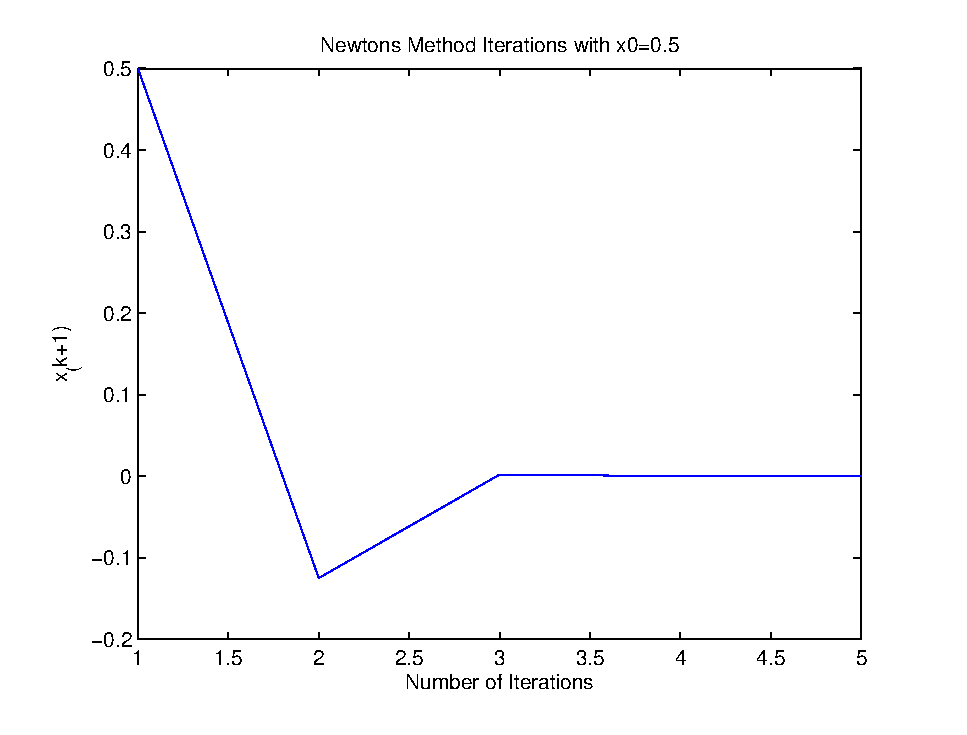
\includegraphics[height=4.5in]{newton1.eps}

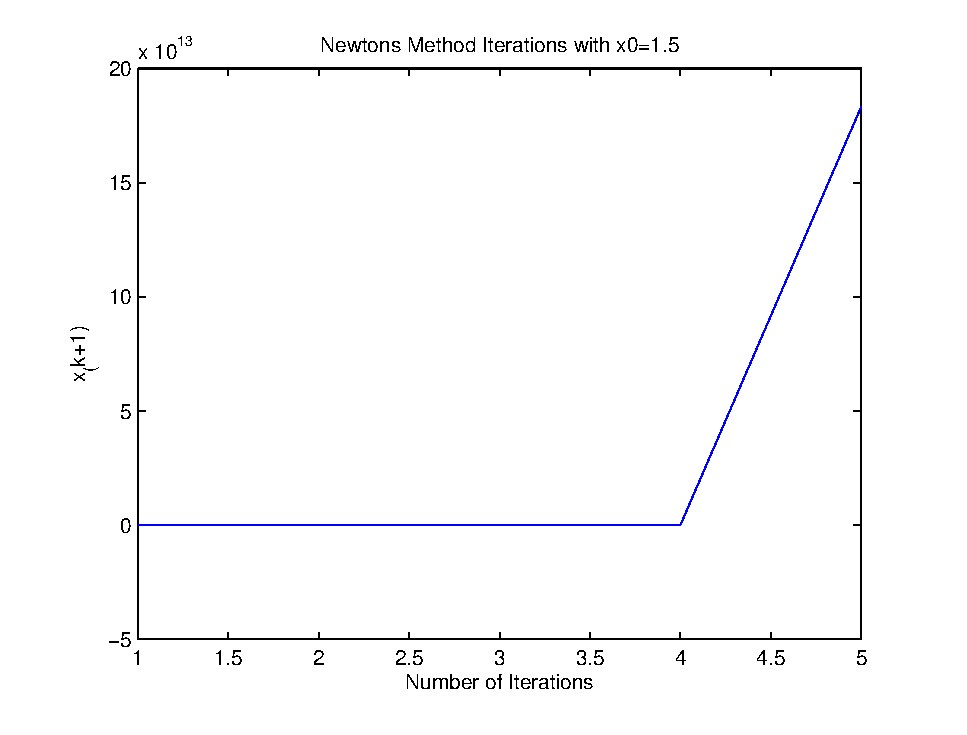
\includegraphics[height=4.5in]{newton2.eps}

\subsection*{Broyden Method Problem}


\subsection*{(i)}
To find the stationary points, we want to solve the equations,
\[
\frac{\partial F(A_{+};\lambda)}{\partial A_{+}} = 0
\]
\[
\frac{\partial F(A_{+};\lambda)}{\partial \lambda} = 0
\]
\[
A_{+}s_{c} =
\begin{bmatrix}
A_{+11} & A_{+12} & \cdots & A_{+1N}\\
A_{+21} & A_{+22} & \cdots &  A_{+2N}\\
\vdots & \vdots &  \ddots & \vdots\\
A_{+N1} & A_{+N2} & \cdots & A_{+NN}\\
\end{bmatrix}
\begin{bmatrix}
s_{c1}\\
s_{c2}\\
\vdots\\
s_{cN}\\
\end{bmatrix} =
\begin{bmatrix}
\sum_{j=1}^N A_{+1j}s_{cj}\\
\sum_{j=1}^N A_{+2j}s_{cj}\\
\vdots\\
\sum_{j=1}^N A_{+Nj}s_{cj}\\
\end{bmatrix}
\]
\newline
\[
\lambda^{T}(A_{+}s_{c}) = 
\begin{bmatrix}
\lambda_{1} & \lambda_{2} & \cdots & \lambda_{N}
\end{bmatrix}
\begin{bmatrix}
\sum_{j=1}^N A_{+1j}s_{cj}\\
\sum_{j=1}^N A_{+2j}s_{cj}\\
\vdots\\
\sum_{j=1}^N A_{+Nj}s_{cj}\\
\end{bmatrix} = \sum_{i=1}^N \sum_{j=1}^N \lambda_{i}A_{+ij}s_{cj}
\]
Fix i, j and take the partial derivative
\begin{align*}
\frac{\partial F(A_{+ij};\lambda)}{\partial A_{+}} &= \frac{\partial}{\partial A_{+ij}} [||A_{+}-A_{c}||_{F}^{2} + \lambda^{T}(A_{+}s_{c}-y{c})]\\
&=\frac{\partial}{\partial A_{+ij}}(\frac{1}{2}\sum_{k=1}^{N} \sum_{l=1}^N (A_{+kl}-A_{c})^{2})+\frac{\partial}{\partial A_{+ij}}(\lambda^{T}(A_{+}s_{c}-y{c}))\\
&= \frac{\partial}{\partial A_{+ij}}(\frac{1}{2}\sum_{k=1}^{N} \sum_{l=1}^N (A_{+kl}-A_{c})^{2})+\frac{\partial}{\partial A_{+ij}}(\lambda^{T}(A_{+}s_{c}))\\
\end{align*}

Since 
\begin{align*}
\frac{\partial}{\partial A_{+ij}}(\frac{1}{2}\sum_{k=1}^{N} \sum_{l=1}^N (A_{+kl}-A_{c})^{2}) &= \sum_{k=1}^N \sum_{l=1}^N \frac{\partial}{\partial A_{+ij}}(\frac{1}{2} (A_{+kl}-A_{ckl})^{2})\\
&= A_{+ij}-A_{cij}
\end{align*}
and similarly,
\begin{align*}
\frac{\partial}{\partial A_{+ij}}(\lambda^{T}(A_{+}s_{c})) &= \frac{\partial}{\partial A_{+ij}} (\sum_{k=1}^N \sum_{l=i}^N \lambda_{k}A_{+kl}s_{cl})\\
&= \sum_{k=1}^N \sum_{l=1}^N [\frac{\partial}{\partial A_{+ij}} (\lambda_{k}A_{+kl}s_{cl})]\\
&= \sum_{k=1}^N \sum_{l=1}^N [\lambda_{k}s_{cl}A_{+kl}]\\
&= \lambda_{i}s_{cj}
\end{align*}
Therefore,
\begin{equation}
\frac{\partial F(A_{+ij};\lambda)}{\partial A_{+ij}} = A_{+ij}-A_{cij}+\lambda_{i}s_{cj}
\end{equation}
\newline
Now fix i and take the partial derivative
\begin{align*}
\frac{\partial F(A_{+};\lambda)}{\partial \lambda} &= \frac{\partial}{\partial \lambda_{i}} [\frac{1}{2} \sum_{k=1}^N \sum_{l=1}^N (A_{+kl}-A_{ckl})^{2}+\sum_{k=1}^N \sum_{l=1}^N \lambda_{k}A_{ckl}s_{cl}-\sum_{k=1}^N\lambda_{k}y_{ck}]\\
&= \frac{\partial}{\partial \lambda_{i}}[\frac{1}{2}\sum_{k=1}^N \sum_{l=1}^N ((A_{ckl}-\lambda_{k}s_{cl})-A_{ckl})^{2} + \sum_{k=1}^N \sum_{l=1}^N \lambda_{k}(A_{ckl}-\lambda_{k}s_{cl})s_{cl} - \sum_{k=1}^N \lambda_{k} y_{ck}]\\
&= \frac{\partial}{\partial \lambda_{i}}[\frac{1}{2}\sum_{k=1}^N \sum_{l=1}^N (\lambda_{k}s_{cl})^{2}] +
\frac{\partial}{\partial \lambda_{i}} [\sum_{k=1}^N \sum_{l=1}^N \lambda_{k}A_{ckl}s_{cl}]- \frac{\partial}{\partial \lambda_{i}}[\sum_{k=1}^N \sum_{l=1}^N \lambda_{k}^{2}s_{cl}^{2}]-\frac{\partial}{\partial \lambda_{i}}[\sum_{k=1}^N \lambda_{k}y_{ck}]\\
&= \sum_{l=1}^N \lambda_{i}s_{cl}^{2} + \sum_{l=1}^N A_{cil}s_{cl} - \sum_{l=1}^N 2\lambda_{i}s_{cl}^{2}-y_{ci}\\
&= -\sum_{l=1}^N \lambda_{i}s_{cl}^{2} + \sum_{l=1}^N A_{cil}s_{cl}-y_{ci}
\end{align*}

Therefore,
\begin{align*}
\frac{\partial F(A_{+};\lambda)}{\partial \lambda} = 0 &\implies -\sum_{l=1}^N \lambda_{i}s_{cl}^{2} + \sum_{l=1}^N A_{cil}s_{cl}-y_{ci} = 0,   \forall i \\ 
& \implies -\lambda s_{c}^{T}s_{c} + A_{c}s_{c}-y_{c} = 0\\
&\implies \lambda s_{c}^{T} = A_{c}s_{c}-y_{c}\\
&\implies \lambda = \frac{A_{c}s_{c}-y_{c}}{s_{c}^{T}s_{c}}
\end{align*}

From equation (1), we have
\begin{align*}
\frac{\partial F(A_{+};\lambda)}{\partial A_{+}} = 0 &\implies A_{+ij} = A_{cij}-\lambda_{i}s_{cj} = 0, \forall i,j\\ &\implies A_{+} = A_{c} - \lambda s_{c}^{T}\\
&\implies A_{+} = A_{c} - \frac{A_{c}s_{c}-y_{c}}{s_{c}^{T}s_{c}} s_{c}^{T}\\
&\implies A_{+} = A_{c} + \frac{1}{s_{c}^{T}s_{c}} (y_{c}-A_{c}s_{c})S_{c}^{T}
\end{align*}

Thus the stationary (critical) points of F in the components of A$_{+}$ and $\lambda$ satisfy
\[
\lambda = \frac{1}{s_{c}^{T}s_{c}}(A_{c}s_{c}-y_{c})
\]
\[
A_{+} = A_{c} + \frac{1}{s_{c}^{T}s_{c}} (y_{c}-A_{c}s_{c})s_{c}^{T}
\]
\subsection*{(ii)}
In order to find the inverse of A+uv$^{T}$, we solve the linear problem (A+uv$^{T}$)x = b. Pre-multiply this equation by A$^{-1}$ 
\begin{equation}
x+A^{-1}uv^{T}x = A^{-1}b 
\end{equation}
\begin{equation}
x = A^{-1}b-A^{-1}uv^{T}x
\end{equation}
\newline
Pre-multiply (2) by v$^{T}$,
\[
v^{T}x + v^{T}A^{-1}uv^{T}x = v^{T}A^{-1}b
\]
\[
v^{T}x(1+v^{T}A^{-1}u) = v^{T}A^{-1}b
\]
\begin{equation}
v^{T}x = \frac{v^{T}A^{-1}b}{1+v^{T}A^{-1}u}
\end{equation}
\newline
Substituting (4) into equation (3), we get
\begin{align*}
x &= A^{-1}b-A^{-1}u(\frac{v^{T}A^{-1}b}{1+v^{T}A^{-1}u})\\
&= (A^{-1}-\frac{A^{-1}uv^{T}A^{-1}}{1+v^{T}A^{-1}u})b
\end{align*}
This implies that 
\[
(A+uv^{T})^{-1} =  A^{-1} - \frac{A^{-1}uv^{T}A^{-1}}{1+v^{T}A^{-1}u}
\]
\newline
The structure of the inverse is clear from noting that A is an invertible matrix, A$^{-1}$uv$^{T}$A$^{-1}$ is a rank one matrix (since uv$^{T}$ is a rank one matrix and any matrix product of a rank one matrix is again a rank one matrix), and 1+v$^{T}$A$^{-1}$u is a scalar. Therefore the inverse of a rank one change to a matrix is the inverse of a matrix subtracted by a rank one matrix.

\subsection*{(iii)}
The first method has operation count of $O(n^{3})$. We show the count line by line below:
\begin{align*}
A_{k}s_{k} &= -f(x_{k})  \text { has $n$ mults $n$ times, and $(n-1)$ adds $n$ times} \implies \text{$O(n^{2})$}\\
x_{k+1} &= x_{k} + s_{k} \text{ has $n$ additions}  \implies \text{$O(n)$}\\
y_k &= f(x_{k+1}) - f(x_k)  \text{ has $n$ subtractions $\implies$ $O(n)$}\\
A_{k+1} &= A_k + \frac{1}{{s_k}^Ts_k} \text{ has } O(n^2) + O(n^2) + O(n) + O(n^2) + O(n^2) \implies O(n^2)
\end{align*}
So there are $O(n^2)$ operations in total. However, note that in order to get $s_k$ in the second line of the algorithm, we must compute ${A_k}^{-1}$ at every iteration, and computing the inverse of a matrix costs $O(n^3)$ operations.

The second method has an identical operation count as the first method and takes $O(n^2)$ time to compute:
\begin{align*}
s_{k} &= {-A_K}^-1f(x_{k})  \text { has $n$ mults $n$ times, and $(n-1)$ adds $n$ times} \implies \text{$O(n^{2})$}\\
x_{k+1} &= x_{k} + s_{k} \text{ has $n$ additions}  \implies \text{$O(n)$}\\
y_k &= f(x_{k+1}) - f(x_k)  \text{ has $n$ subtractions $\implies$ $O(n)$}\\
{A_{k+1}}^{-1} &= {A_k}^{-1} + \frac{s_k - {A_k}^{-1}y_k}{{s_k}^T{A_k}^{-1}y_k}{s_k}^T{A_k}^{-1} \text{ has a bunch of $O(n^2)$ counts} \implies O(n^2)
\end{align*}
Since the matrix ${A_k}^{-1}$ is directly computed, the Sherman-Morrison method only takes $O(n^2)$ operations to run. The inverse matrix must still be found, but it only needs to be computed once at the start of the algorithm.

\subsection*{(iv)}
Matlab code for Newton's and Broyden's Method 
\begin{lstlisting}
function [newton newtonCounter broyden broydenCounter nResults bResults] = hw3_q3()

    % Fix sigma = 1, rho = 2, beta = 1
    sigma = 1;
    rho = 2;
    beta = 1;
   
    % Find fixed points
    p = sqrt(beta*(rho-1));
    fixedPoint1 = [0 0 0];
    fixedPoint2 = [p p rho-1];
    fixedPoint3 = [-p -p rho-1];
    
    % Starting points
    initial = (-1.5:0.1:1.5)';
    initialPoints = [initial initial zeros(length(initial),1)];
    
    newton = [];
    newtonCounter = [];
    
    % Newton's method
    for i=1:length(initial)
         [a b c] = Newton(sigma, rho, beta, initialPoints(i,:));
         newton = [newton; a];
         newtonCounter = [newtonCounter; b];
    end
    
    broyden = [];
    broydenCounter = [];
    
    % Broyden's method
    for i=1:length(initial)
         [a b] = Broyden(sigma, rho, beta, initialPoints(i,:));
         broyden = [broyden; a];
         broydenCounter = [broydenCounter; b];
    end
    
    % Compare Newton and Broyden for the last starting point calculated
    [a b c] = Newton(sigma, rho, beta, initialPoints(length(initial),:));
    nResults = analyzeError(a, c);
    [a b c] = Broyden(sigma, rho, beta, initialPoints(2,:));
    bResults = analyzeError(a, c);
end

function [answer] = analyzeError(solution, steps)
    answer = [];
    
    for i=1:length(steps)
        residual = abs(solution - steps(i,:));
        answer = [answer; norm(residual, 2)];
    end
end

% Multi-dimensional Newton's method
function [answer counter results] = Newton(sigma, rho, beta, initialGuess)

    xk = initialGuess;
    fxk = F(sigma, rho, beta, xk);
    fxk = fxk'*fxk; % use dot product to test if fxk is the zero vector
    
    results = xk; % store every intermediate step
    
    % iterate until the solution is found
    counter = 0;
    while fxk ~= 0
        
        xk = NewtonStep(sigma, rho, beta, xk);
        fxk = F(sigma, rho, beta, xk);
        fxk = fxk'*fxk;
        
        if counter > 50
            break
        end
        
        counter = counter+1;
        results = [results; xk];
    end
    answer = xk;
end

function [answer] = NewtonStep(sigma, rho, beta, xk)
    f = F(sigma, rho, beta, xk);
    jacobian = JacobianF(sigma, rho, beta, xk);
    answer = (jacobian\(-f+(jacobian*xk')))';
end

% Broyden's method
function [answer counter results] = Broyden(sigma, rho, beta, initialGuess)
    AkInverse = JacobianF(sigma, rho, beta, initialGuess);
    xk = initialGuess;
    fxk = F(sigma, rho, beta, xk);
    fxk = fxk'*fxk;
    
    results = xk; % store every intermediate step
    
    counter = 0;
    while fxk ~=0
        
        [xk AkInverse] = BroydenStep(sigma, rho, beta, xk, AkInverse);
        fxk = F(sigma, rho, beta, xk);
        fxk = fxk'*fxk;
        
        if counter > 100
            break
        end
        
        counter = counter+1;
        
        results = [results; xk];
    end
    answer = xk;
end

% Use Sherman-Morrison's formula to calculate the next step
function [nextStep nextMatrix] = BroydenStep(sigma, rho, beta, xk, AkInverse)
    sk = -AkInverse*F(sigma, rho, beta, xk);
    xk = xk';
    
    xknext = xk + sk;
    yk = F(sigma, rho, beta, xknext) - F(sigma, rho, beta, xk);
    nextMatrix = AkInverse + ((sk-AkInverse*yk)/(sk'*AkInverse*yk))*sk'*AkInverse;
    nextStep = xknext';
end

% Lorenz equations
function [answer] = F(sigma, rho, beta, xk)
    x = xk(1);
    y = xk(2);
    z = xk(3);
    answer = [sigma*(y-x) rho*x-y-x*z -beta*z+x*y]';
end

% Jacobian of Lorenz equations
function [answer] = JacobianF(sigma, rho, beta, xk)
    x = xk(1);
    y = xk(2);
    z = xk(3);
    answer = [-sigma sigma 0; rho-z -1 -x; y x -beta];
end
\end{lstlisting}

\begin{lstlisting}
Q3
Newton's method converges to different roots depending on starting guess.

newton =

    -1    -1     1
    -1    -1     1
    -1    -1     1
    -1    -1     1
    -1    -1     1
    -1    -1     1
    -1    -1     1
    -1    -1     1
     1     1     1
     0     0     0
     0     0     0
     0     0     0
     0     0     0
     0     0     0
     0     0     0
     0     0     0
     0     0     0
     0     0     0
     0     0     0
     0     0     0
     0     0     0
     0     0     0
    -1    -1     1
     1     1     1
     1     1     1
     1     1     1
     1     1     1
     1     1     1
     1     1     1
     1     1     1
     1     1     1

Broyden's method converges to different roots depending on starting guess.

broyden =

  -1.000000000000000  -1.000000000000000   1.000000000000000
  -1.000000000000000  -1.000000000000000   1.000000000000000
  -1.000000000000000  -1.000000000000000   1.000000000000000
  -1.000000000000000  -1.000000000000000   1.000000000000000
  -1.000000000000000  -1.000000000000000   1.000000000000000
                 NaN                 NaN                 NaN (-1,-1,0)
   1.000000000000000   1.000000000000000   1.000000000000000
  -1.000000000000000  -1.000000000000000   1.000000000000000
  -0.000000000000000  -0.000000000000000  -0.000000000000000
  -0.000000000000000  -0.000000000000000  -0.000000000000000
  -0.000000000000000  -0.000000000000000  -0.000000000000000
   0.000000000000000   0.000000000000000   0.000000000000000
  -0.000000000000000  -0.000000000000000  -0.000000000000000
   0.000000000000000   0.000000000000000   0.000000000000000
  -0.000000000000000  -0.000000000000000  -0.000000000000000
                   0                   0                   0
   0.000000000000000   0.000000000000000  -0.000000000000000
  -0.000000000000000  -0.000000000000000   0.000000000000000
   0.000000000000000   0.000000000000000  -0.000000000000000
  -0.000000000000000  -0.000000000000000   0.000000000000000
   0.000000000000000   0.000000000000000  -0.000000000000000
   0.000000000000000   0.000000000000000  -0.000000000000000
   0.000000000000000   0.000000000000000  -0.000000000000000
   1.000000000000000   1.000000000000000   1.000000000000000
  -1.000000000000000  -1.000000000000000   1.000000000000000
                 NaN                 NaN                 NaN (1,1,0)
   1.000000000000000   1.000000000000000   1.000000000000000
   1.000000000000000   1.000000000000000   1.000000000000000
   1.000000000000000   1.000000000000000   1.000000000000000
   1.000000000000000   1.000000000000000   1.000000000000000
   1.000000000000000   1.000000000000000   1.000000000000000

previous error is approximately next error squared => quadratic convergence

nResults =

   1.224744871391589
   0.360696604941503
   0.021244012082731
   0.000225733738193
   0.000000028802302
   0.000000000000001
                   0

previous error is approximately next error ^ 1.25 => superlinear convergence
bResults =

   1.224744871391589
   5.557933518853928
   2.473452147460146
   6.647662861397232
   4.869955240818563
  23.117651921082057
   2.491054239499819
   1.588295695632145
   0.744663853822398
   0.588162470972346
   0.506844645249347
   0.411022685642346
   0.017496185311085
   0.076336423953497
   0.030195262949251
   0.004481926652841
   0.000416454596790
   0.000027421821391
   0.000001198372470
   0.000000013062352
   0.000000000180630
   0.000000000006115
   0.000000000000014
                   0

bResults =

   0.200000000000000   0.200000000000000   1.000000000000000
   1.000000000000000   3.128000000000000   1.000000000000000
   0.471480314960630   0.920779527559056   1.000000000000000
   1.395878360740666   1.893317525561743   0.057907431119938
   0.313372190826388   1.125726448674978   2.030208596141200
   0.306221684265671   2.028006517450967   4.618016833397222
   0.128972664557071   0.057252584718051   0.527637083397019
   0.068030480227793   0.008079140621570   0.214189562217368
   0.024687574867902   0.008297118760277   0.070955286935565
   0.005183583487847   0.002656950354130   0.013470187667776
   0.000922253528386   0.000340055445875   0.002481836435865
   0.000106528930290   0.000026281200580   0.000324864772537
   0.000014027543130   0.000002647343127   0.000038817561860
   0.000000498269975   0.000000061436608   0.000001091823911
   0.000000010195466   0.000000020555048   0.000000012107447
   0.000000001187452   0.000000002964954   0.000000002423284
   0.000000000011279   0.000000000023882   0.000000000015403
   0.000000000000048   0.000000000000111   0.000000000000082
   0.000000000000000   0.000000000000000   0.000000000000000
                   0                   0                   0
\end{lstlisting}
\clearpage
Matlab code to calculate convergence rate for Newton's and Broyden's Method
\begin{lstlisting}
function [convergenceRate] = convergence(resultArray)

convergenceRate = [];
for i=2:length(resultArray)
    convergence = log(resultArray(i))/log(resultArray(i-1));
    convergenceRate = [convergenceRate convergence];
end
end
\end{lstlisting}

Convergence rate for Broyden's Method at each iteration:
\begin{lstlisting}
ans =

   1.545026792091282
   1.439379005544468
   1.349503034994076
   1.298012532273264
   1.331436439136100
   1.235824016167096
   1.150914678297556
   1.235452271573459
\end{lstlisting}
From above result, we can confirm that the convergence rate for Broyden's method is approximately 1.25, which is superlinear but subquadratic. 

Convergence rate for Newton's Method at each iteration:
\begin{lstlisting}
ans =

   2.179867992711640
   2.067947978250778
   1.989238801533066
\end{lstlisting}
Again, from above we can confirm that the convergence rate for Newton's method is quadratic. 



\subsection*{(extra credit)}
Matlab Code 
\begin{lstlisting}
function [varyBeta counterB determinantB errorB1 errorB2 varyRho counterR determinantR errorR1 errorR2] = extraCredit()

    % Fix sigma = 1, rho = 2, beta = 1
    sigma = 1;
    rho = 2:-0.1:1;
    beta = 1:-0.1:0;
    
    varyBeta = [1 1 1];
    counterB = [0];
    
    fixedB = [];
    % get the actual answer
    for i=1:length(beta)
        fixedB = [fixedB; findFixedPoint(rho(1), beta(i))];
    end
    
    fixedR = [];
    for i=1:length(rho)
        fixedR = [fixedR; findFixedPoint(rho(i), beta(1))];
    end
    fixedB
    fixedR
    
    % We know that initially there is a solution at (1,1,1)
    for i=2:length(beta)
        
        [a b] = Newton(sigma, rho(1), beta(i), varyBeta(i-1,:));
        varyBeta = [varyBeta; a];
        counterB = [counterB; b];
    end
    
    determinantB = [];
    % calculate the determinant of the jacobian
    for i=1:length(varyBeta)
        temp = det(JacobianF(sigma, rho(1), beta(i), varyBeta(i,:)));
        determinantB = [determinantB; temp];
    end
    
    % compare residuals of beta=0.9 and beta=0
    [a b c] = Newton(sigma, rho(1), beta(2), varyBeta(1,:));
    errorB1 = analyzeError(findFixedPoint(2,0.9), c);
    temp = length(varyBeta)-1;
    [a b c] = Newton(sigma, rho(1), 0, varyBeta(temp,:));
    errorB2 = analyzeError(findFixedPoint(rho(1),0),c);
    
    % Repeat same study but on rho
    varyRho = [1 1 1];
    counterR = [0];
    for i=2:length(rho)
        
        [a b] = Newton(sigma, rho(i), beta(1), varyRho(i-1,:));
        varyRho = [varyRho; a];
        counterR = [counterR; b];
        
    end
    
    determinantR = [];
    for i=1:length(varyRho)
        temp = det(JacobianF(sigma, rho(i), beta(1), varyRho(i,:)));
        determinantR = [determinantR; temp];
    end
    
    [a b c] = Newton(sigma, rho(2), beta(1), varyRho(1,:));
    errorR1 = analyzeError(findFixedPoint(rho(2), beta(1)), c);
    [a b c] = Newton(sigma, rho(length(rho)), beta(1), varyRho(length(rho)-1,:));
    errorR2 = analyzeError(findFixedPoint(rho(length(rho)), (beta(1))), c);
end

function[answer] = findFixedPoint(rho, beta)
    answer = [sqrt(beta*(rho-1)) sqrt(beta*(rho-1)) rho-1];
end

% takes absolute value of intermediate step - actual root
function [answer] = analyzeError(solution, steps)
    answer = [];
    for i=1:length(steps)
        residual = abs(solution - steps(i,:));
        answer = [answer; residual];
    end
end
\end{lstlisting}

\begin{lstlisting}

Actual solutions:
Beta =

   1.000000000000000   1.000000000000000   1.000000000000000
   0.948683298050514   0.948683298050514   1.000000000000000
   0.894427190999916   0.894427190999916   1.000000000000000
   0.836660026534076   0.836660026534076   1.000000000000000
   0.774596669241483   0.774596669241483   1.000000000000000
   0.707106781186548   0.707106781186548   1.000000000000000
   0.632455532033676   0.632455532033676   1.000000000000000
   0.547722557505166   0.547722557505166   1.000000000000000
   0.447213595499958   0.447213595499958   1.000000000000000
   0.316227766016838   0.316227766016838   1.000000000000000
                   0                   0   1.000000000000000
                   
Rho =

   1.000000000000000   1.000000000000000   1.000000000000000
   0.948683298050514   0.948683298050514   0.900000000000000
   0.894427190999916   0.894427190999916   0.800000000000000
   0.836660026534076   0.836660026534076   0.700000000000000
   0.774596669241483   0.774596669241483   0.600000000000000
   0.707106781186548   0.707106781186548   0.500000000000000
   0.632455532033676   0.632455532033676   0.400000000000000
   0.547722557505166   0.547722557505166   0.300000000000000
   0.447213595499958   0.447213595499958   0.200000000000000
   0.316227766016838   0.316227766016838   0.100000000000000
                   0                   0                   0

Approximations:
Beta =

   1.000000000000000   1.000000000000000   1.000000000000000
   0.948683298050514   0.948683298050514   1.000000000000000
   0.894427190999916   0.894427190999916   1.000000000000000
   0.836660026534076   0.836660026534076   1.000000000000000
   0.774596669241483   0.774596669241483   1.000000000000000
   0.707106781186547   0.707106781186547   1.000000000000000
   0.632455532033676   0.632455532033676   1.000000000000000
   0.547722557505166   0.547722557505166   1.000000000000000
   0.447213595499958   0.447213595499958   1.000000000000000
   0.316227766016838   0.316227766016838   1.000000000000000
   0.000000000000000   0.000000000000000   1.000000000000000

varyRho =
Note that the very last estimation is incorrect.

   1.000000000000000   1.000000000000000   1.000000000000000
   0.948683298050514   0.948683298050514   0.900000000000000
   0.894427190999916   0.894427190999916   0.800000000000000
   0.836660026534075   0.836660026534075   0.700000000000000
   0.774596669241484   0.774596669241484   0.600000000000000
   0.707106781186548   0.707106781186548   0.500000000000000
   0.632455532033676   0.632455532033676   0.400000000000000
   0.547722557505166   0.547722557505166   0.300000000000000
   0.447213595499958   0.447213595499958   0.200000000000000
   0.316227766016838   0.316227766016838   0.100000000000000
   0.000000008788027   0.000000008788027   0.000000000000000

Determinant of Jacobian from beta = 1 to beta = 0
-2.000000000000000
-1.800000000000000
-1.600000000000000
-1.400000000000000
-1.200000000000000
-1.000000000000000
-0.800000000000000
-0.600000000000000
-0.400000000000000
-0.200000000000000
-0.000000000000000

Significant digits Newton at beta = 0.9

Note that the number of significant digits roughly doubles each iteration
0.051316701949486   0.051316701949486                   0
0.001316701949486   0.001316701949486                   0
0.000000912475802   0.000000912475802                   0
0.000000000000439   0.000000000000439                   0

Significant digits Newton at beta = 0

With a singular matrix, the number of digits increases extremely slowly
0.316227766016838   0.316227766016838                   0
0.158113883008419   0.158113883008419                   0
0.079056941504209   0.079056941504209                   0
0.039528470752105   0.039528470752105                   0
0.019764235376052   0.019764235376052                   0
0.009882117688026   0.009882117688026                   0
0.004941058844013   0.004941058844013                   0
0.002470529422007   0.002470529422007                   0
0.001235264711003   0.001235264711003                   0
0.000617632355502   0.000617632355502                   0
0.000308816177751   0.000308816177751                   0
0.000154408088875   0.000154408088875                   0
0.000077204044438   0.000077204044438                   0
0.000038602022219   0.000038602022219                   0
0.000019301011109   0.000019301011109                   0
0.000009650505555   0.000009650505555                   0
0.000004825252777   0.000004825252777                   0
0.000002412626389   0.000002412626389                   0
0.000001206313194   0.000001206313194                   0
0.000000603156597   0.000000603156597                   0
0.000000301578299   0.000000301578299                   0
0.000000150789149   0.000000150789149                   0
0.000000075394575   0.000000075394575                   0
0.000000037697287   0.000000037697287                   0
0.000000018848644   0.000000018848644                   0
0.000000009424322   0.000000009424322                   0
0.000000004712161   0.000000004712161                   0
0.000000002356080   0.000000002356080                   0
0.000000001178040   0.000000001178040                   0
0.000000000589020   0.000000000589020                   0
0.000000000294510   0.000000000294510                   0
0.000000000147255   0.000000000147255                   0
0.000000000073628   0.000000000073628                   0
0.000000000036814   0.000000000036814                   0
0.000000000018407   0.000000000018407                   0
0.000000000009203   0.000000000009203                   0
0.000000000004602   0.000000000004602                   0
0.000000000002301   0.000000000002301                   0
0.000000000001150   0.000000000001150                   0
0.000000000000575   0.000000000000575                   0
0.000000000000288   0.000000000000288                   0
0.000000000000144   0.000000000000144                   0
0.000000000000072   0.000000000000072                   0
0.000000000000036   0.000000000000036                   0
0.000000000000018   0.000000000000018                   0
0.000000000000009   0.000000000000009                   0
0.000000000000004   0.000000000000004                   0
0.000000000000002   0.000000000000002                   0
0.000000000000001   0.000000000000001                   0
0.000000000000001   0.000000000000001                   0
0.000000000000000   0.000000000000000                   0

Determinant of Jacobian from rho = 2 to rho = 1
-2.000000000000000
-1.800000000000000
-1.600000000000000
-1.400000000000000
-1.200000000000001
-1.000000000000000
-0.800000000000000
-0.600000000000000
-0.400000000000000
-0.200000000000000
-0.000000000000000

Significant digits Newton at rho = 1.9

Again the number of significant digits roughly doubles each iteration
0.051316701949486   0.051316701949486   0.100000000000000
0.003697654330439   0.003697654330439   0.004761904761905
0.000016840276853   0.000016840276853   0.000018404070268
0.000000000321639   0.000000000321639   0.000000000326683
0.000000000000000   0.000000000000000   0.000000000000000

Significant digits Newton at rho = 1
Again with a singular matrix, convergence takes much longer
0.316227766016838   0.316227766016838   0.100000000000000
0.210818510677892   0.210818510677892   0.033333333333333
0.134157234067749   0.134157234067749   0.012121212121212
0.083976283920271   0.083976283920271   0.004533888503354
0.052202240080312   0.052202240080312   0.001715484007459
0.032349843891895   0.032349843891895   0.000652394765408
0.020018572855516   0.020018572855516   0.000248683013799
0.012379512794689   0.012379512794689   0.000094897098421
0.007653103004907   0.007653103004907   0.000036231036103
0.004730502829800   0.004730502829800   0.000013836065239
0.002923793870860   0.002923793870860   0.000005284373337
0.001807057186976   0.001807057186976   0.000002018354856
0.001116838283385   0.001116838283385   0.000000770925616
0.000690248548253   0.000690248548253   0.000000294464256
0.000426598385063   0.000426598385063   0.000000112474774
0.000263652687122   0.000263652687122   0.000000042961439
0.000162946434460   0.000162946434460   0.000000016409791
0.000100706467765   0.000100706467765   0.000000006267979
0.000062240029858   0.000062240029858   0.000000002394154
0.000038466456892   0.000038466456892   0.000000000914486
0.000023773577819   0.000023773577819   0.000000000349302
0.000014692879494   0.000014692879494   0.000000000133422
0.000009080698925   0.000009080698925   0.000000000050963
0.000005612184636   0.000005612184636   0.000000000019466
0.000003468523688   0.000003468523688   0.000000000007435
0.000002143660512   0.000002143660512   0.000000000002840
0.000001324850039   0.000001324850039   0.000000000001085
0.000000818804881   0.000000818804881   0.000000000000414
0.000000506032506   0.000000506032506   0.000000000000158
0.000000312710518   0.000000312710518   0.000000000000060
0.000000193297481   0.000000193297481   0.000000000000023
0.000000119563354   0.000000119563354   0.000000000000009
0.000000073867264   0.000000073867264   0.000000000000003
0.000000045951779   0.000000045951779   0.000000000000001
0.000000028186490   0.000000028186490   0.000000000000000
0.000000017524664   0.000000017524664   0.000000000000000
0.000000010392296   0.000000010392296   0.000000000000000
0.000000008490951   0.000000008490951   0.000000000000000

\end{lstlisting}

\end{document}  